\chapter{Introduction}

\section{Motivation}
Sound has been a subject of fascination for a long time and with good reason. We have known since prehistoric times that sound travels slower than light, evermore proven whenever a flash of lightning was seen before the clap was heard \cite{ampel1993history}.  In 1636AD, Marin Mersènne of Paris used a pendulum to make speed of sound measurements by firing cannons. The $\rom{19}^{th}$ century mark the first attempts to create transducers and Graham Bell invention of the phone in 1876 mark a clear step forward in the technology allowing to transmit intelligible sounds. While the transducer technology was slowly developing, the inability to process the data limited the development of sound localization tool. The beginnings of sound localization can be trace back during the $\rom{20}^{th}$ century war, when rudimentary systems were developed to localize incoming enemy airplanes, giant rotating waveguides were used by an operator to steer and amplify the sound arriving from a given direction, the prequel of beamforming. For a long time, ears were the only tool to localize sound, until the development of computer and array signal processing techniques. Sound localization technology has matured since then and is now part of our daily life and implemented in countless products such as hearing aid, headset, etc.. making our life much easier in the end. This technology can now be used to solve new problems such as accessing the impact of environmental noise on human. This impact is still been studied by researchers around the world \footnote{some study claim that sound can cause health issue. Regulation are still being written to quantify a safe daily noise exposure} and a reliable noise monitoring system is yet to be developed to detect the main noise contributors in an outdoor environment. This thesis tackle the problem of localizing and quantifying main noise disturbance in outdoor environment. The main challenges of sound localization arise in developing a robust technique to localize multiple sources in a changing complex outdoor sound field. This thesis propose a method to solve this problem.

\section{Background}

Sound localization algorithms have been successfully applied (to varying degrees) to a wide range of engineering problems. Traditionally, distinction is usually made between algorithm using the time difference of arrival (TDOA) of signal between pairs microphones to find the position of a source and the algorithm using beamforming Steered Response Power (SRP). However, the SRP-PHAT algorithm, one of the most robust and widely implemented technique combines the advantages of those two techniques. A significant bit of research has been done on implementing SRP-PHAT on speech enhancement systems, whereby speaker identification and teleconferencing in an environment having high background noise and reverberant conditions was needed. Outdoor sound can be appreciably different from this situation. This thesis propose to adapt SRP-PHAT to outdoor multisources sound localization. 

\begin{figure}[H]
    \centering
    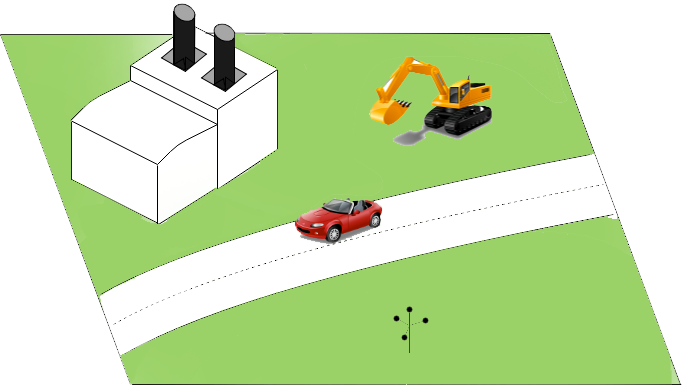
\includegraphics[width=0.8\textwidth]{Figures/scenario33.png}
    \caption{sketch of the proposed case solved by the thesis}
    \label{fig:Introductioncase}
\end{figure}

\section{Scope and outline of the thesis}

This thesis focus mainly on source signal spectrum ranging from low-to-mid frequencies in the far field. It should be noted that the purpose of this thesis is not to track moving sources, rather the thesis tackles the problem of \textit{static outdoor sound levels and their contributors} with the constraint of using as few microphones as possible while being robust to different noise and weather conditions. The thesis propose a solution capable of retrieving the noise source position in a variety of scenario including free-field to moderate reverberating environments. While previous research mostly tackle the problem of single source localization using linear or circular arrays, this thesis use a tetrahedral array to capture the signals.

The organization of the thesis is as follow: chapter 2 derives the theory used to analyze the problem and create our simulation framework. Chapter 3 focus on describing the methods employed to solve the problem as well as algorithm features and its robustness and performance in outdoor conditions the algorithm performance.
Chapter 4 contains experimental results, anechoic and outdoor measurements investigating the algorithm limits in a variety of scenario.
Chapter 5 encompass a discussion about the solution and propose new ideas and further work.




